% Author: Marek Fiser <tikz at marekfiser.cz>
% MESIF protocol: http://en.wikipedia.org/wiki/MESIF_protocol
\documentclass[tikz, border=10pt]{standalone}
%%%<
\usepackage{verbatim}
\usetikzlibrary{calc}
\usetikzlibrary{fit}
%%%>
\begin{comment}
:Title: MESIF protocol
:Tags: Diagrams;Block diagrams;Computer science
:Author: Marek Fiser
:Slug: mesif

A diagram describing the MESIF protocol: http://en.wikipedia.org/wiki/MESIF_protocol
\end{comment}
\usetikzlibrary{arrows}
\begin{document}
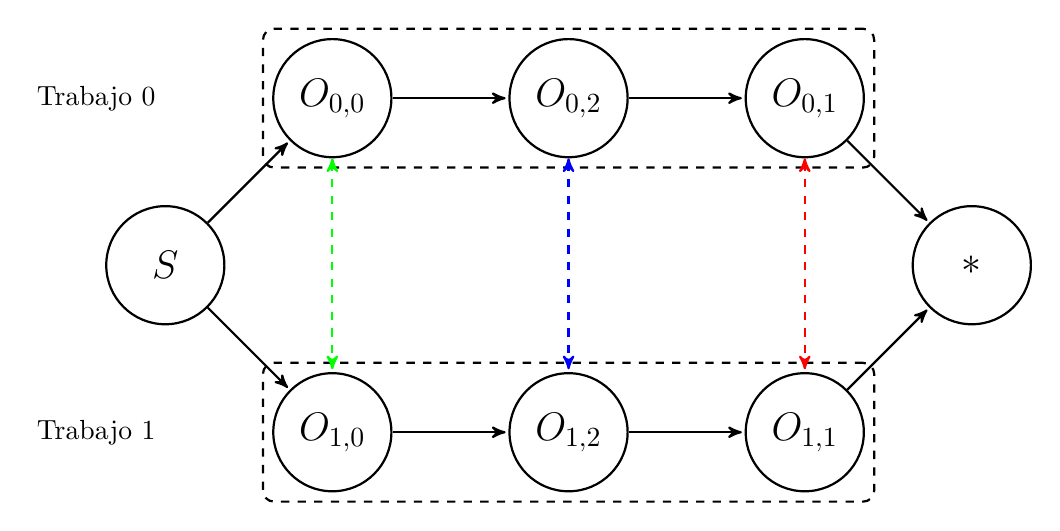
\begin{tikzpicture}[->,>=stealth',shorten >=1pt,auto,node distance=3cm,
  thick,main node/.style={circle,fill=white!20,draw,
  font=\sffamily\Large\bfseries,minimum size=15mm}]
  \node[main node] (j00) {$O_{0,0}$}; 
  \node[main node] (j01)[right of=j00] {$O_{0,2}$};
  \node[main node] (j02)[right of=j01] {$O_{0,1}$};
  \node[main node] (S)[below left of=j00] {$S$};
  \node[main node] (j10) [below right of= S]{$O_{1,0}$}; 
  \node[main node] (j11)[right of=j10] {$O_{1,2}$};
  \node[main node] (j12)[right of=j11] {$O_{1,1}$};
  \node[main node] (s) [above right of=j12]{$\ast$};
  \node (t0)[left of=j00]{Trabajo 0};
  \node (t1)[left of=j10]{Trabajo 1};
  \node[draw,dashed,rounded corners,fit= (j00) (j01) (j02)]{};
  \node[draw,dashed,rounded corners,fit= (j10) (j11) (j12)]{};

  \path[every node/.style={font=\sffamily\small,
  		fill=white,inner sep=1pt}]
  	% Right-hand-side arrows rendered from top to bottom to
  	% aristas

  	(S) edge node {} (j00)
  	(S) edge node {} (j10)
  	(j00) edge node {}(j01)
  	(j01) edge node {}(j02)
  	(j10) edge node{} (j11)
  	(j11) edge node {}(j12)
  	(j12) edge node {} (s)
  	(j02) edge node {} (s)	
  	(j00) edge[dashed,<->,green] node {}(j10)
  	(j02) edge[dashed,<->,red] node {}(j12)
  	(j01) edge[dashed,<->,blue] node {}(j11);


%    (M) edge [-] node {} (E)
%    (S) edge [dashed,-] node {} (F)
%    (E) edge [dashed,-] node {} (S)
%    (F) edge [-] node {} (I)
%    (I) edge [-] node{} (JSI)
%    (I) edge [-] node {} (JSI);
    % flechas de movimimiento 
    %(M) edge [bend left=30] node{} (E)
%    \path(M) edge [bend left=150] node[left=10mm,above=1mm]{} (S)
%	(E) edge [bend left=150] node{} (M);   
%    
%    \path(I) edge [bend left=150] node[left=10mm,above=1mm]{} (S)
%	(F) edge [bend left=150] node{} (I);   
%    
%    %\path (E) edge [bend left=150] node[above=1mm] {backward} (I)
%    %(I) edge [bend left=150] node{backward} (E);
%
%     \node[draw,rounded corners,fit=(M) (E) (S) (F) (I)] {};
  	% Left-hand-side arrows rendered from bottom to top to
  	% achieve proper rendering of labels over arrows.
%    (I) edge [bend left=65] node[left=1mm] {PrWr/BusRdX} (M)
%        edge [bend left=55] node[left=1mm] {PrRd/BusRd Ex} (E)
%        edge [bend left=30] node[left=1mm] {PrRd/BusRd} (F)
%    (F) edge [loop above] node {PrRd/-} (F)
%        edge [bend left=50] node[left=1mm] {PrWr/BusRdX} (M)
%        edge [bend left=30] node[left=1mm] {BusRd/Flush} (S)
%    (S) edge [bend left=40] node[left=1mm] {PrWr/BusRdX} (M)
%    (E) edge [bend left=30] node[left=1mm] {PrWr/-} (M);
\end{tikzpicture}
\end{document}
